%----------------------------------------------------------------------------
%bb defines the bounding box for the pdf
%viewport defines the area of the pdf used
%in sidewaysfigure the last entry in bb moves the caption toward/away the pic
%in sidewaysfigure the second entry in bb moves the pic toward/away the caption
%----------------------------------------------------------------------------
\begin{figure}
\scalebox{0.7}[0.7]{
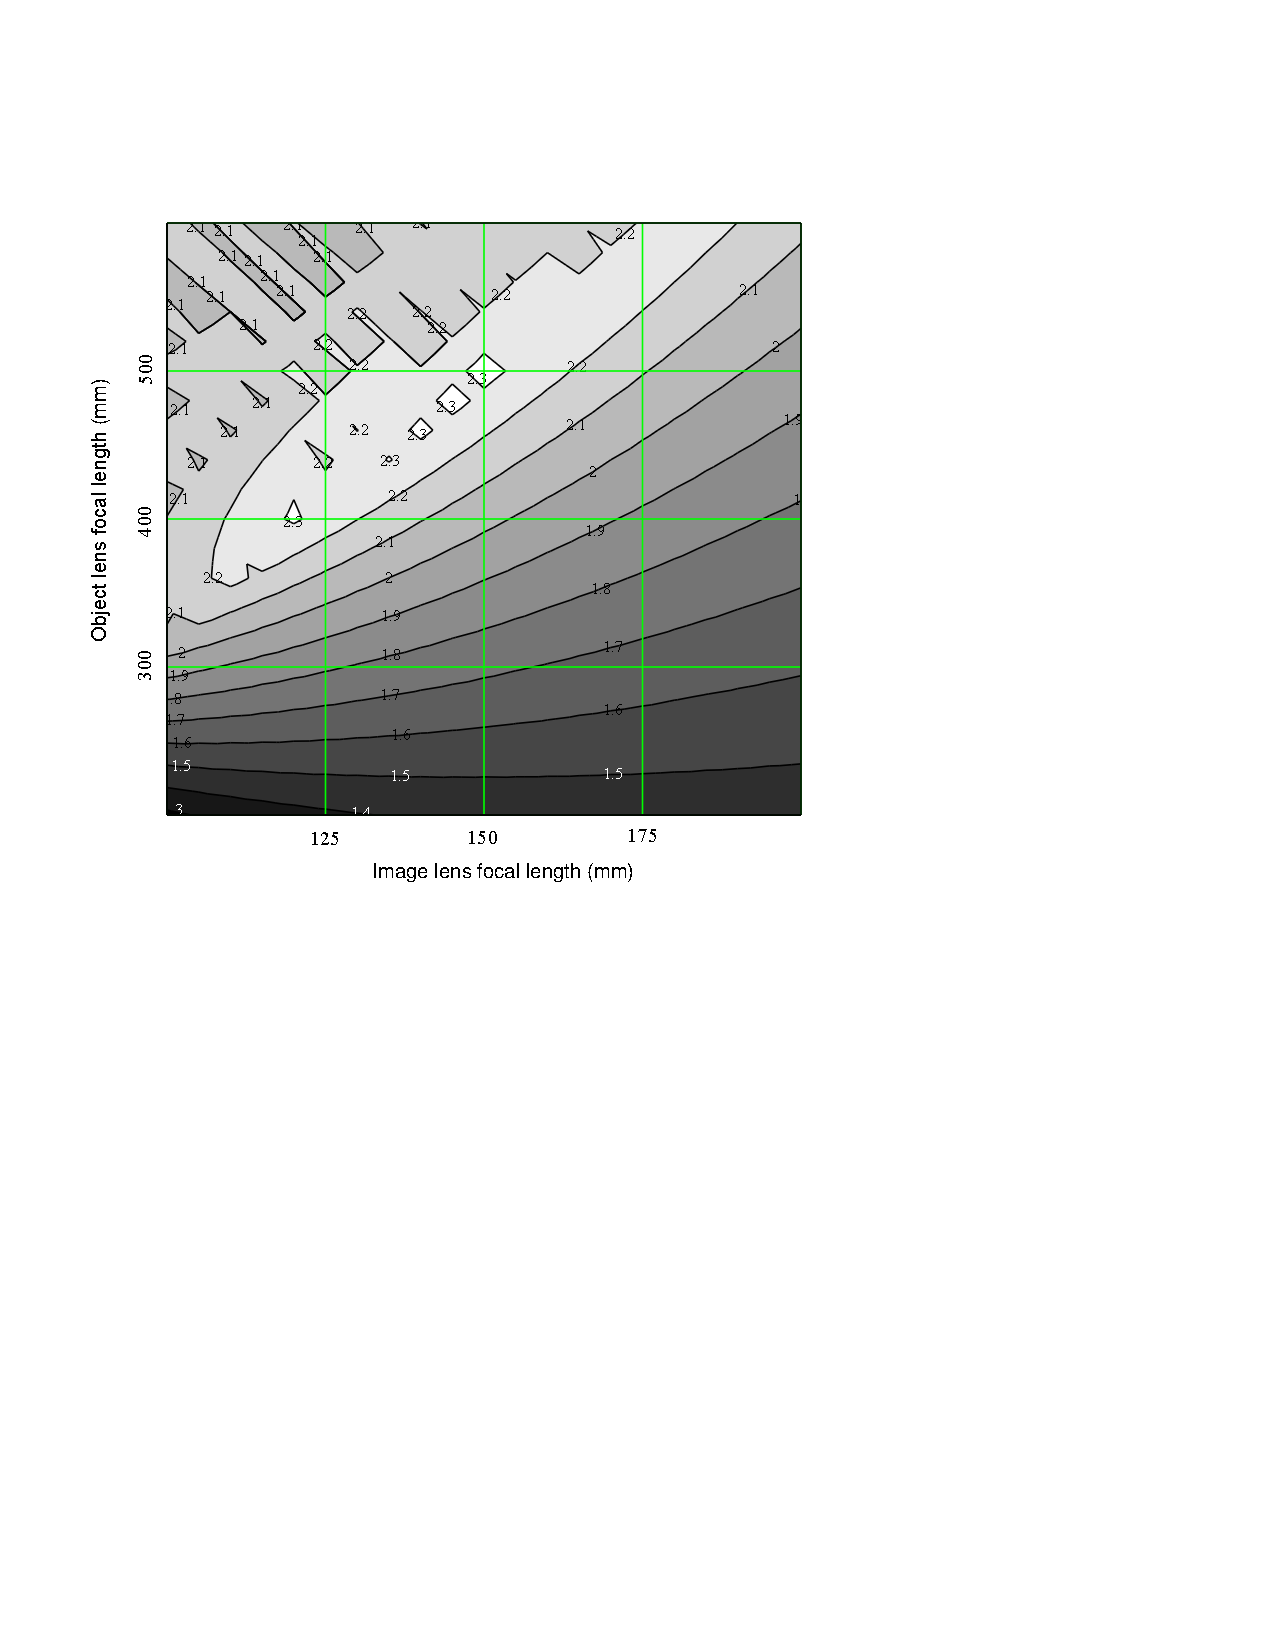
\includegraphics[bb=-60 360 489 725]
{side_view/side_view.pdf}
}
\caption[Side--view lens optimization surface]{Side--view lens optimization surface. For this calculation the beam waist diameter is 1 mm, the wavelength is 0.63 $\mu$m, the slitwidth is 300 $\mu$m, the slit height is 0.5 cm, and the monochromator acceptance angle is 52 mrad. The object lens is placed one focal length from the sample, while the image lens is placed one focal length from the monochromator input. The units for the contour in the plot are $10^{-12}$ m$^3$ (scaled volume). Thus if the target was air (near $10^{25}$ molecules per cubic meter) we would expect this system to be sensitive to $10^{13}$ atmospheric molecules (assuming all molecules decay optically in an isotropic fashion).}
\label{side_view}
\end{figure}
%----------------------------------------------------------------------------
